\chapter{free field theory}
\section{partition function}
\begin{itemize}
	\item 考虑标量场
	\begin{equation}
		\mathcal{L} = - \frac{1}{2} (\partial \phi)^2 - V(\phi),
	\end{equation}
	A. Zee: 在作用量里, 时间的导数项必须是正的, 包括标量场的 $(\partial_0 \phi)^2$ 和电磁场的 $(\partial_0 A_i)^2$.
	
	\item 含有 source function 的路径积分为
	\begin{equation}
		Z(J) = \int D\phi \, e^{i \int d^d x \, (- \frac{1}{2} (\partial \phi)^2 - V(\phi) + J(x) \phi(x))}.
	\end{equation}
	
	\item 当 $V(\phi) = \frac{1}{2} m^2 \phi^2$ 时, 称作 free or Gaussian theory.
	
	\noindent\rule[0.5ex]{\linewidth}{0.5pt} % horizontal line
	
	\item 计算 free theory 的 partition function, 得到
	\begin{equation} \label{free field theory.1.3}
		Z(J) = \mathcal{C} e^{- \frac{i}{2} \int d^d x d^d y \, J(x) D(x - y) J(y)},
	\end{equation}
	另外, 用 $W(J)$ 表示指数上的部分 (去除掉虚数 $i$).
	
	\begin{tcolorbox}[title=proof:]
		注意 $\partial^\mu \phi \partial_\mu \phi = \partial^\mu(\phi \partial_\mu \phi) - \phi \partial^2 \phi$, 忽略全微分项, 那么
		\begin{equation} \label{free field theory.1.4}
			Z(J) = \int D\phi \, e^{i \int d^d x \, (\frac{1}{2} \phi (\partial^2 - m^2) \phi + J(x) \phi(x))},
		\end{equation}
		代入 \eqref{Gaussian integrals and Gaussian-Berezin integrals.1.1}, 可知
		\begin{equation}
			Z(J) = \mathcal{C} e^{- \frac{i}{2} \int d^d x d^d y \, J(x) D(x - y) J(y)},
		\end{equation}
		其中 $D(x - y)$ 满足
		\begin{equation} \label{free field theory.1.6}
			\begin{dcases}
				(\partial^2 - m^2) D(x - y) = \delta^{(d)}(x - y) \\
				(- p^2 - m^2) \tilde{D}(p, q) = (2 \pi)^d \delta^{(d)}(p - q)
			\end{dcases} \Longrightarrow D(x - y) = \int \frac{d^d k}{(2 \pi)^d} \frac{e^{i k \cdot (x - y)}}{- k^2 - m^2}.
		\end{equation}
	\end{tcolorbox}
\end{itemize}

\section{free propagator}
\begin{itemize}
	\item 为了使 \eqref{free field theory.1.4} 中的积分在 $\phi$ 较大时收敛, 作替换 $m^2 \mapsto m^2 - i \epsilon$, 这样被积函数中会出现一项 $e^{- \epsilon \int d^d x \phi^2}$.
	
	\item 注意 \eqref{free field theory.1.6} 中的积分会遇到奇点, 必须加入正无穷小量 $\epsilon$ 避免发散,
	\begin{equation} \label{free field theory.2.1}
		D(x) = \int \frac{d^d k}{(2 \pi)^d} \frac{e^{i k \cdot x}}{- k^2 - m^2 + i \epsilon} = - i \int \frac{d^D k}{(2 \pi)^D 2 \omega_k} \Big( \theta(t) e^{i (- \omega_k t + \vec{k} \cdot \vec{x})} + \theta(- t) e^{i (\omega_k t + \vec{k} \cdot \vec{x})} \Big).
	\end{equation}
	
	\begin{tcolorbox}[title=calculation:]
		对 $k^0$ 积分, 注意有两个奇点 $k^0 = \pm (\omega_k - i \epsilon)$, 当 $t > 0$ 时, contour 处于下半平面, ... (另外注意到我们可以任意改变 $\vec{k}$ 的符号).
		
		取 $D = 3$, 可以尝试在球坐标下继续计算, 考虑 $\theta(t)$ 项,
		\begin{align}
			i I(x) &= \frac{1}{(2 \pi)^3} \int_0^\pi \sin \theta d\theta \int_0^{2 \pi} d\phi \int_0^\infty k^2 dk \, \frac{e^{- i (\omega_k t - k r \cos \theta)}}{2 (k^2 + m^2)} \notag \\
			&= \frac{1}{(2 \pi)^2 r} \frac{1}{2 i} \int_{- \infty}^{+ \infty} \frac{k}{k^2 + m^2} e^{- i (\omega_k t - k r)} dk,
		\end{align}
		注意到 $k = \pm i m$ 既是极点也是 branch cut 的顶点.
		
		\begin{figure}[H]
			\centering
			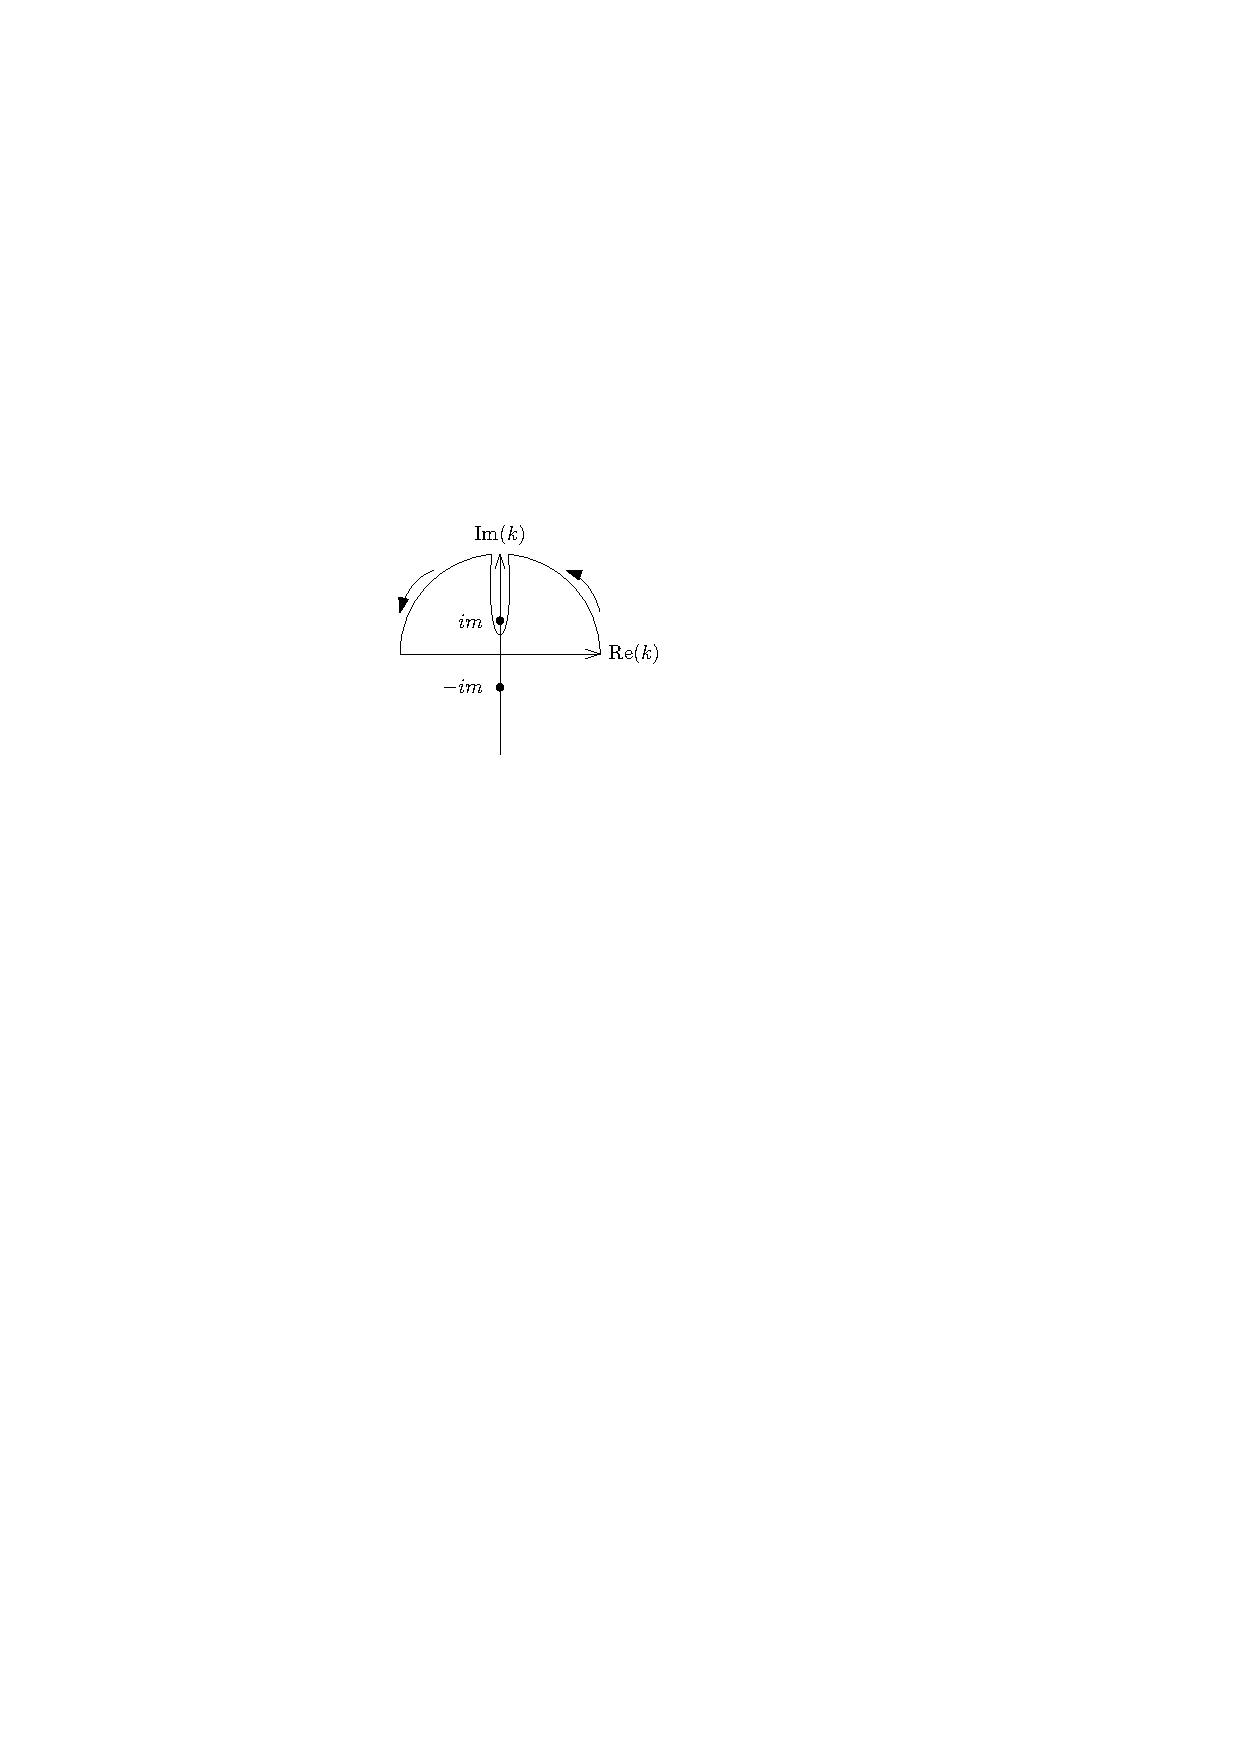
\includegraphics[scale=1]{figures/contour for evaluating the integral of the free field propagator.pdf}
			\caption{contour for evaluating the integral of the free field propagator.}
		\end{figure}
		
		参考 figure \ref{graph of sqrt{1 + z^2}.}, 可知 $\omega_k$ 在 branch cut 两侧的取值分别为
		\begin{equation}
			\omega_k = \begin{dcases}
				i \sqrt{\kappa^2 - m^2} & k = \pm (i \kappa + 0^+) \\
				- i \sqrt{\kappa^2 - m^2} & k = \pm (i \kappa + 0^-)
			\end{dcases},
		\end{equation}
		其中 $\kappa > m$. 注意到 $\theta(t)$ 决定了 $t > 0$, 那么 contour 的两个上半平面的弧中, 左侧的弧对积分不贡献, 但右侧的弧在 $t > r$ (类时) 情况下会发散, 在 $t < r$ (类空) 的情况下才收敛到零.
	\end{tcolorbox}
	
	\item $D(x)$ 的取值与 $x$ 的类时, 类空性质关系密切.
	\begin{itemize}
		\item 类时区域,
		\begin{equation}
			D(t, 0) = - i \int \frac{d^D k}{(2 \pi)^D 2 \omega_k} \Big( \theta(t) e^{- i \omega_k t} + \theta(- t) e^{i \omega_k t} \Big).
		\end{equation}
		
		\item 类空区域,
		\begin{equation}
			D(0, \vec{x}) = - i \int \frac{d^D k}{(2 \pi)^D 2 \omega_k} e^{i \vec{k} \cdot \vec{x}} \sim e^{- m |\vec{x}|}.
		\end{equation}
	\end{itemize}
\end{itemize}

\section{from field to particle to force}
\subsection{from field to particle}
\begin{itemize}
	\item 考虑 \eqref{free field theory.1.3} 中的 $W(J)$,
	\begin{align}
		W(J) &= - \frac{1}{2} \int d^d x d^d y \, J(y) D(x - y) J(y) \\
		&= - \frac{1}{2} \int \frac{d^d k}{(2 \pi)^d} \tilde{J}(- k) \frac{1}{- k^2 - m^2 + i \epsilon} \tilde{J}(k),
	\end{align}
	其中, 如果 $J(x)$ 是实函数, 那么 $\tilde{J}(- k) = \tilde{J}^*(k)$.
	
	\noindent\rule[0.5ex]{\linewidth}{0.5pt} % horizontal line
	
	\item 考虑 $J(x) = J_1(x) + J_2(x)$, 那么 $W(J)$ 共有 4 项, 其中一个交叉项如下,
	\begin{equation}
		W_{1 2}(J) = - \frac{1}{2} \int \frac{d^d k}{(2 \pi)^d} \tilde{J}_1(- k) \frac{1}{- k^2 - m^2 + i \epsilon} \tilde{J}_2(k),
	\end{equation}
	可见 $W(J)$ 取值较大的条件是:
	\begin{enumerate}
		\item $\tilde{J}_1(k), \tilde{J}_2(k)$ 有较大重叠,
		
		\item 重叠位置的 $k$ 是 on shell (即 $k^2 = - m^2$).
	\end{enumerate}
	
	\item 可以看出来, 这里有一个粒子从 1 传递到 2 \textcolor{red}{(?)}.
\end{itemize}

\subsection{from particle to force}
\begin{itemize}
	\item 考虑 $J(x) = \delta^{(D)}(\vec{x} - \vec{x}_1) + \delta^{(D)}(\vec{x} - \vec{x}_1) \Longrightarrow \tilde{J}_a(k) = 2 \pi e^{- i \vec{k} \cdot \vec{x}_a} \delta(k^0)$, 那么
	\begin{align}
		W_{1 2}(J) + W_{2 1}(J) &= \delta(0) \int \frac{d^D k}{(2 \pi)^{D - 1}} \frac{1}{|\vec{k}|^2 + m^2 - i \epsilon} \cos(\vec{k} \cdot (\vec{x}_1 - \vec{x}_2)) \notag \\
		&\overset{D = 3}{=} 2 \pi \delta(0) \frac{1}{4 \pi r} e^{- m r}, \label{free field theory.3.4}
	\end{align}
	($- i \epsilon$ 显然可以舍去), 注意到 $\braket{0 | e^{- i H T} | 0} = e^{- i E T}$, 而时间间隔 $T = \int dx^0 = 2 \pi \delta(0)$, 所以
	\begin{equation}
		E = - \frac{W(J)}{T} \overset{D = 3}{=} - \frac{1}{4 \pi r} e^{- m r}.
	\end{equation}
	
	\begin{tcolorbox}[title=calculation:]
		计算 \eqref{free field theory.3.4} 中的积分, 令 $\vec{x}_1 - \vec{x}_2 = \vec{r}$,
		\begin{align}
			I_D &= \int \frac{d^D k}{(2 \pi)^D} \frac{1}{|\vec{k}|^2 + m^2} \overbrace{\cos(\vec{k} \cdot \vec{r})}^{\mapsto e^{i \vec{k} \cdot \vec{r}}} \notag \\
			&= \frac{1}{(2 \pi)^D} \int (k \sin \theta_1)^{D - 2} d\Omega_{D - 2} \int k d\theta_1 dk \, \frac{1}{k^2 + m^2} e^{i k r \cos \theta_1} \notag \\
			&= \frac{S_{D - 2}}{(2 \pi)^D} \int k^{D - 1} \sin^{D - 2} \theta_1 d\theta_1 dk \, \frac{1}{k^2 + m^2} e^{i k r \cos \theta_1},
		\end{align}
		取 $D = 3$, 那么
		\begin{align}
			I_{D = 3} &= \frac{1}{(2 \pi)^2} \int k^2 \sin \theta_1 d\theta_1 dk \, \frac{1}{k^2 + m^2} e^{i k \cos \theta_1} \notag \\
			&= \frac{1}{2 \pi^2 r} \int_0^\infty \sin(k r) \frac{k dk}{k^2 + m^2} = \frac{- i}{4 \pi^2 r} \int_{- \infty}^\infty e^{i k r} \frac{k dk}{k^2 + m^2} \notag \\
			&= \frac{- i}{4 \pi^2 r} 2 \pi i \, \underbrace{\mathrm{Res}(f, i m)}_{= \frac{1}{2} e^{- m r}} = \frac{1}{4 \pi r} e^{- m r}.
		\end{align}
	\end{tcolorbox}
\end{itemize}

\section{vacuum energy} \label{free field theory.4}
\begin{itemize}
	\item 注意到
	\begin{equation} \label{free field theory.4.1}
		Z(J = 0) = \braket{0 | e^{- i H T} | 0},
	\end{equation}
	所以
	\begin{equation}
		E_0 = \braket{0 | H | 0} = V \int \frac{d^D k}{(2 \pi)^D} \frac{1}{2} \omega_k + \text{irrelevant terms}.
	\end{equation}
	
	\begin{tcolorbox}[title=calculation:]
		代入 \eqref{Gaussian integrals and Gaussian-Berezin integrals.1.1} (其中 $N$ 是时空格点总数),
		\begin{equation}
			Z(J = 0) = (2 \pi)^{\frac{N}{2}} (\det A)^{- \frac{1}{2}},
		\end{equation}
		其中 $A = - i (\partial^2 - m^2 + i \epsilon)$.
		\begin{itemize}
			\item 注意到 $\det e^A = e^{\mathrm{tr} \, A} \Longrightarrow \det A = e^{\mathrm{tr} \, \ln A}$, 代入, 并有
			\begin{equation}
				(\ln A) \phi(x) = \int \frac{d^d k}{(2 \pi)^d} e^{i k \cdot x} \ln(- i (- k^2 - m^2 + i \epsilon)) \tilde{\phi}(k),
			\end{equation}
			对于 $A : v \mapsto u$ 以及变换 $P : v \mapsto \tilde{v}$, 有 $P A P^{- 1} : \tilde{v} \mapsto \tilde{u}$, 且 $\mathrm{tr} \, A = \mathrm{tr} \, P A P^{- 1}$, 所以
			\begin{align}
				- \frac{1}{2} \mathrm{tr} \, \ln A &= - \frac{1}{2} \mathrm{tr} \, \ln(- i (- k^2 - m^2 + i \epsilon)) \notag \\
				&= - \frac{1}{2} \sum_k \ln(- i (- k^2 - m^2 + i \epsilon)) \notag \\
				&= - \frac{1}{2} \frac{V T}{(2 \pi)^d} \int d^d k \, \ln(- i (- k^2 - m^2 + i \epsilon)),
			\end{align}
			其中, 参考 \eqref{Dirac delta function & Fourier transformation.2.5}, 有 $\sum_k = \frac{V T}{(2 \pi)^d} \int d^d k$.
		\end{itemize}
		
		代入 \eqref{free field theory.4.1},
		\begin{align}
			E_0 &= \frac{i}{T} \Big( \frac{N}{2} \ln (2 \pi) - \frac{1}{2} \frac{V T}{(2 \pi)^d} \int d^d k \, \ln(- i (- k^2 - m^2 + i \epsilon)) \Big) \notag \\
			&= \frac{i N}{2 T} \ln (2 \pi) - \frac{i}{2} V \int \frac{d^d k}{(2 \pi)^d} \Big( \ln(\underbrace{- k^2 - m^2 + i \epsilon}_{= (k^0)^2 - \omega_k^2 + i \epsilon}) - \frac{\pi}{2} i \Big),
		\end{align}
		略去与 $m$ 无关的常数项
		\begin{equation}
			\frac{\Delta E_0}{V} = - \frac{i}{2} \int \frac{d^D k}{(2 \pi)^D} \int \frac{dk^0}{2 \pi} \ln((k^0)^2 - \omega_k^2 + i \epsilon),
		\end{equation}
		做分部积分,
		\begin{equation}
			\ln((k^0)^2 - \omega_k^2 + i \epsilon) = \frac{d}{dk^0} (k^0 \ln((k^0)^2 - \omega_k^2 + i \epsilon)) - k^0 \frac{2 k^0}{(k^0)^2 - \omega_k^2 + i \epsilon},
		\end{equation}
		代入,
		\begin{align}
			\frac{E_0}{V} &= \frac{i}{2} \int \frac{d^D k}{(2 \pi)^D} \int \frac{dk^0}{2 \pi} \frac{2 (k^0)^2}{(k^0)^2 - \omega_k^2 + i \epsilon} \notag \\
			&= \frac{i}{2} \int \frac{d^D k}{(2 \pi)^D} \Big( \frac{1}{2 \pi} 2 \pi i \frac{2 (- \omega_k)^2}{- 2 \omega_k} \Big) = \int \frac{d^D k}{(2 \pi)^D} \frac{1}{2} \omega_k.
		\end{align}
		另外, $\ln(z^2 - 1 + i \epsilon)$ 的图像如下:
		
		\begin{figure}[H]
			\centering
			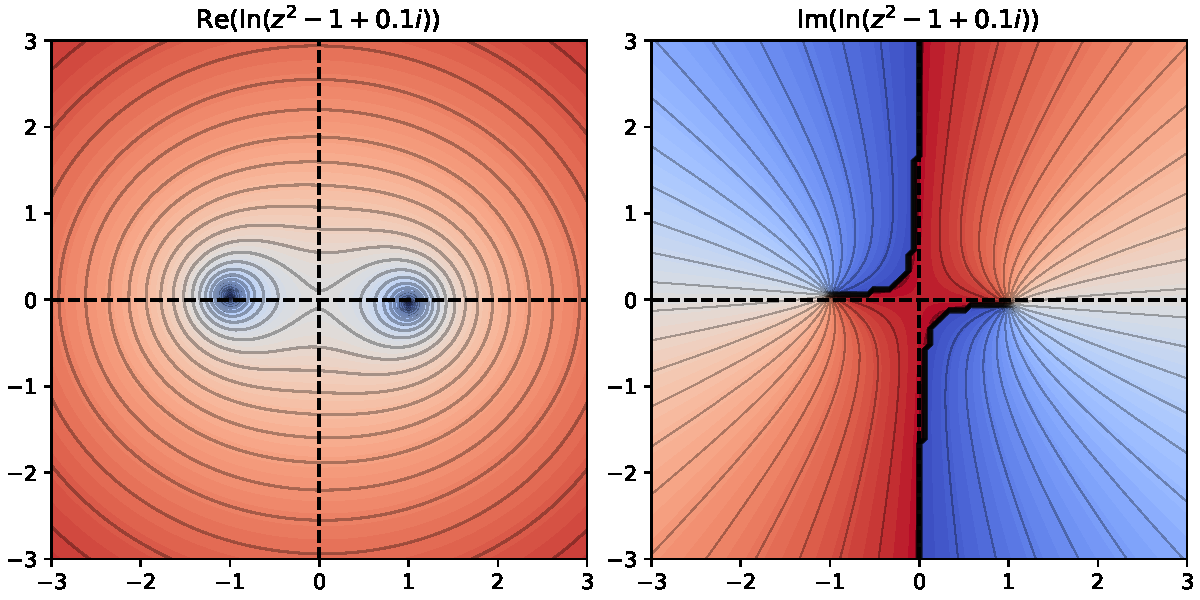
\includegraphics[scale=0.5]{figures/ln(z^2 - 1 + i epsilon).pdf}
			\caption{graph of $\ln(z^2 - 1 + i \epsilon)$.}
		\end{figure}
	\end{tcolorbox}
\end{itemize}
